% \begin{savequote}[8cm]
% \textlatin{Neque porro quisquam est qui dolorem ipsum quia dolor sit amet, consectetur, adipisci velit...}

% There is no one who loves pain itself, who seeks after it and wants to have it, simply because it is pain...
%   \qauthor{--- Cicero's \textit{de Finibus Bonorum et Malorum}}
% \end{savequote}

\chapter{\label{ch:1-intro}Introduction} 

\minitoc
\newpage

Proteins are the molecular building blocks of all living systems. The emergence of life from these fundamental components depends on how proteins are organised in both space and time, and across a magnitude of scales. Understanding the forces governing this organisation not only elucidates how matter comes alive, but knowing how and why these processes go wrong can help us to design effective therapeutics for disease or even hijack and engineer these processes to harness the power of proteins.

In this thesis I explore three different mechanisms for protein organisation. I will develop mathematical models that capture the main features of physical interactions between proteins and study the structure and consequences of these equations, comparing with experimental studies where relevant. Each mechanism has broadly been studied before but I will detail how previous studies have failed to capture key features of the interaction that can lead to a fundamentally different route for protein organisation.

\section{What is a protein}

Proteins are a class of biomolecules that are long unbranched chains of monomer units, called amino acids. \cite{jones2002soft} Each amino acid has the same basic structure that polymerises to form a protein backbone held together by peptide bonds, a type of covalent bond. The distinct amino acids have distinct side chains that are attached to the polymerising unit and it is this side chain that defines the different amino acids. This sequence of amino acids, including their side chains, defines the protein and is referred to as the primary protein structure. An array of non-covalent bonds, such as hydrogen bonds, electrostatic attractions and van der Waals, further define the 3D configuration of the chain in giving the protein a secondary and ternary structure. This ternary structure defines the shape of the protein,  and specifies the location of each atom, although thermal fluctuations induce slight perturbations and prevent proteins from being fixed in this exact configuration. The protein's ternary structure is also crucial in determining the proteins function, for example proteins that catalyse biological reactions, enzymes, do so by binding to a molecule to form a complex. The lock and key model of this binding requires that the enzyme and molecule have exactly complimentary shapes.

these interactions are fundamentally encoded into the DNA o.. information of life

and often the protein's functions specifically depends on this structure which is exactly defined by the genetic information. This is the central dogma of biology: DNA makes RNA, and RNA makes proteins.

The genetic information in an organism's DNA encode for the sequence of amino acids that define the protein. Proteins are manufactured by connected this sequence of amino acids by covalent bonds and this is called the primary protein structure.

Specificity research to try and improve the effect of catalysts to speed up reactions.

Quaternary structure, beyond single proteins we get groups -> can be scaled up to larger enzyme complexes (channelling? perhaps)

Proteins are the work horses of cellular and subcellular machinery. Enzymes are proteins that catalyse reactions, making processes feasible on relevant molecular timescales. Kinesin and other motor proteins drag cargo and provide essential active transport functionality, however proteins such as ion channels can span barriers within the cell and allow passive transport to occur moving. This aresenal of transport processes determines how the distribution of biomolecules is kept from equilibrium, or how efficiently a system can relax to some steady state, helping to control cell signalling and the flow of information. Another function of proteins is as building blocks for subcellular structures such as microtubules or viral capsids \cite{keskin_principles_2008}. If anything happens on the scale of \todo{quantify this scale somehow...} there is normally a protein making to happen.

lots of discussion around sepcificity of enzyme to exact shape of some substrates etc.

phosphorylation of proteins

\begin{figure}
    \centering
    % 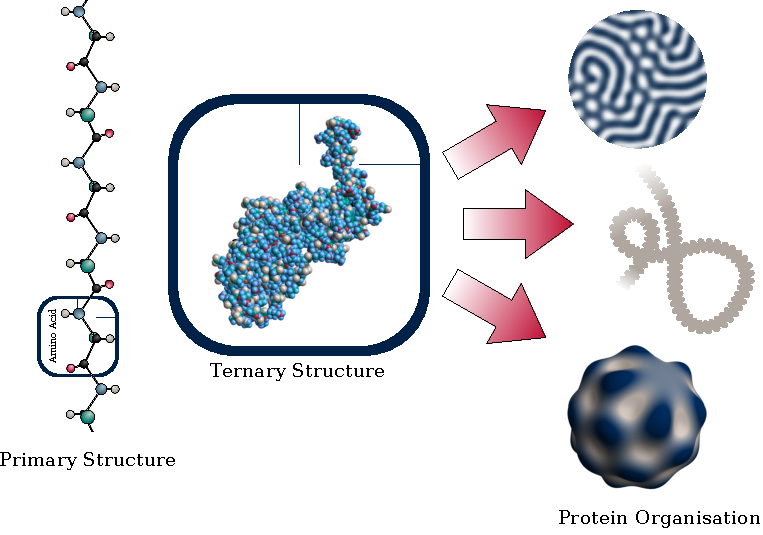
\includegraphics[width=0.8\textwidth]{figures/proteinLevels.pdf}
    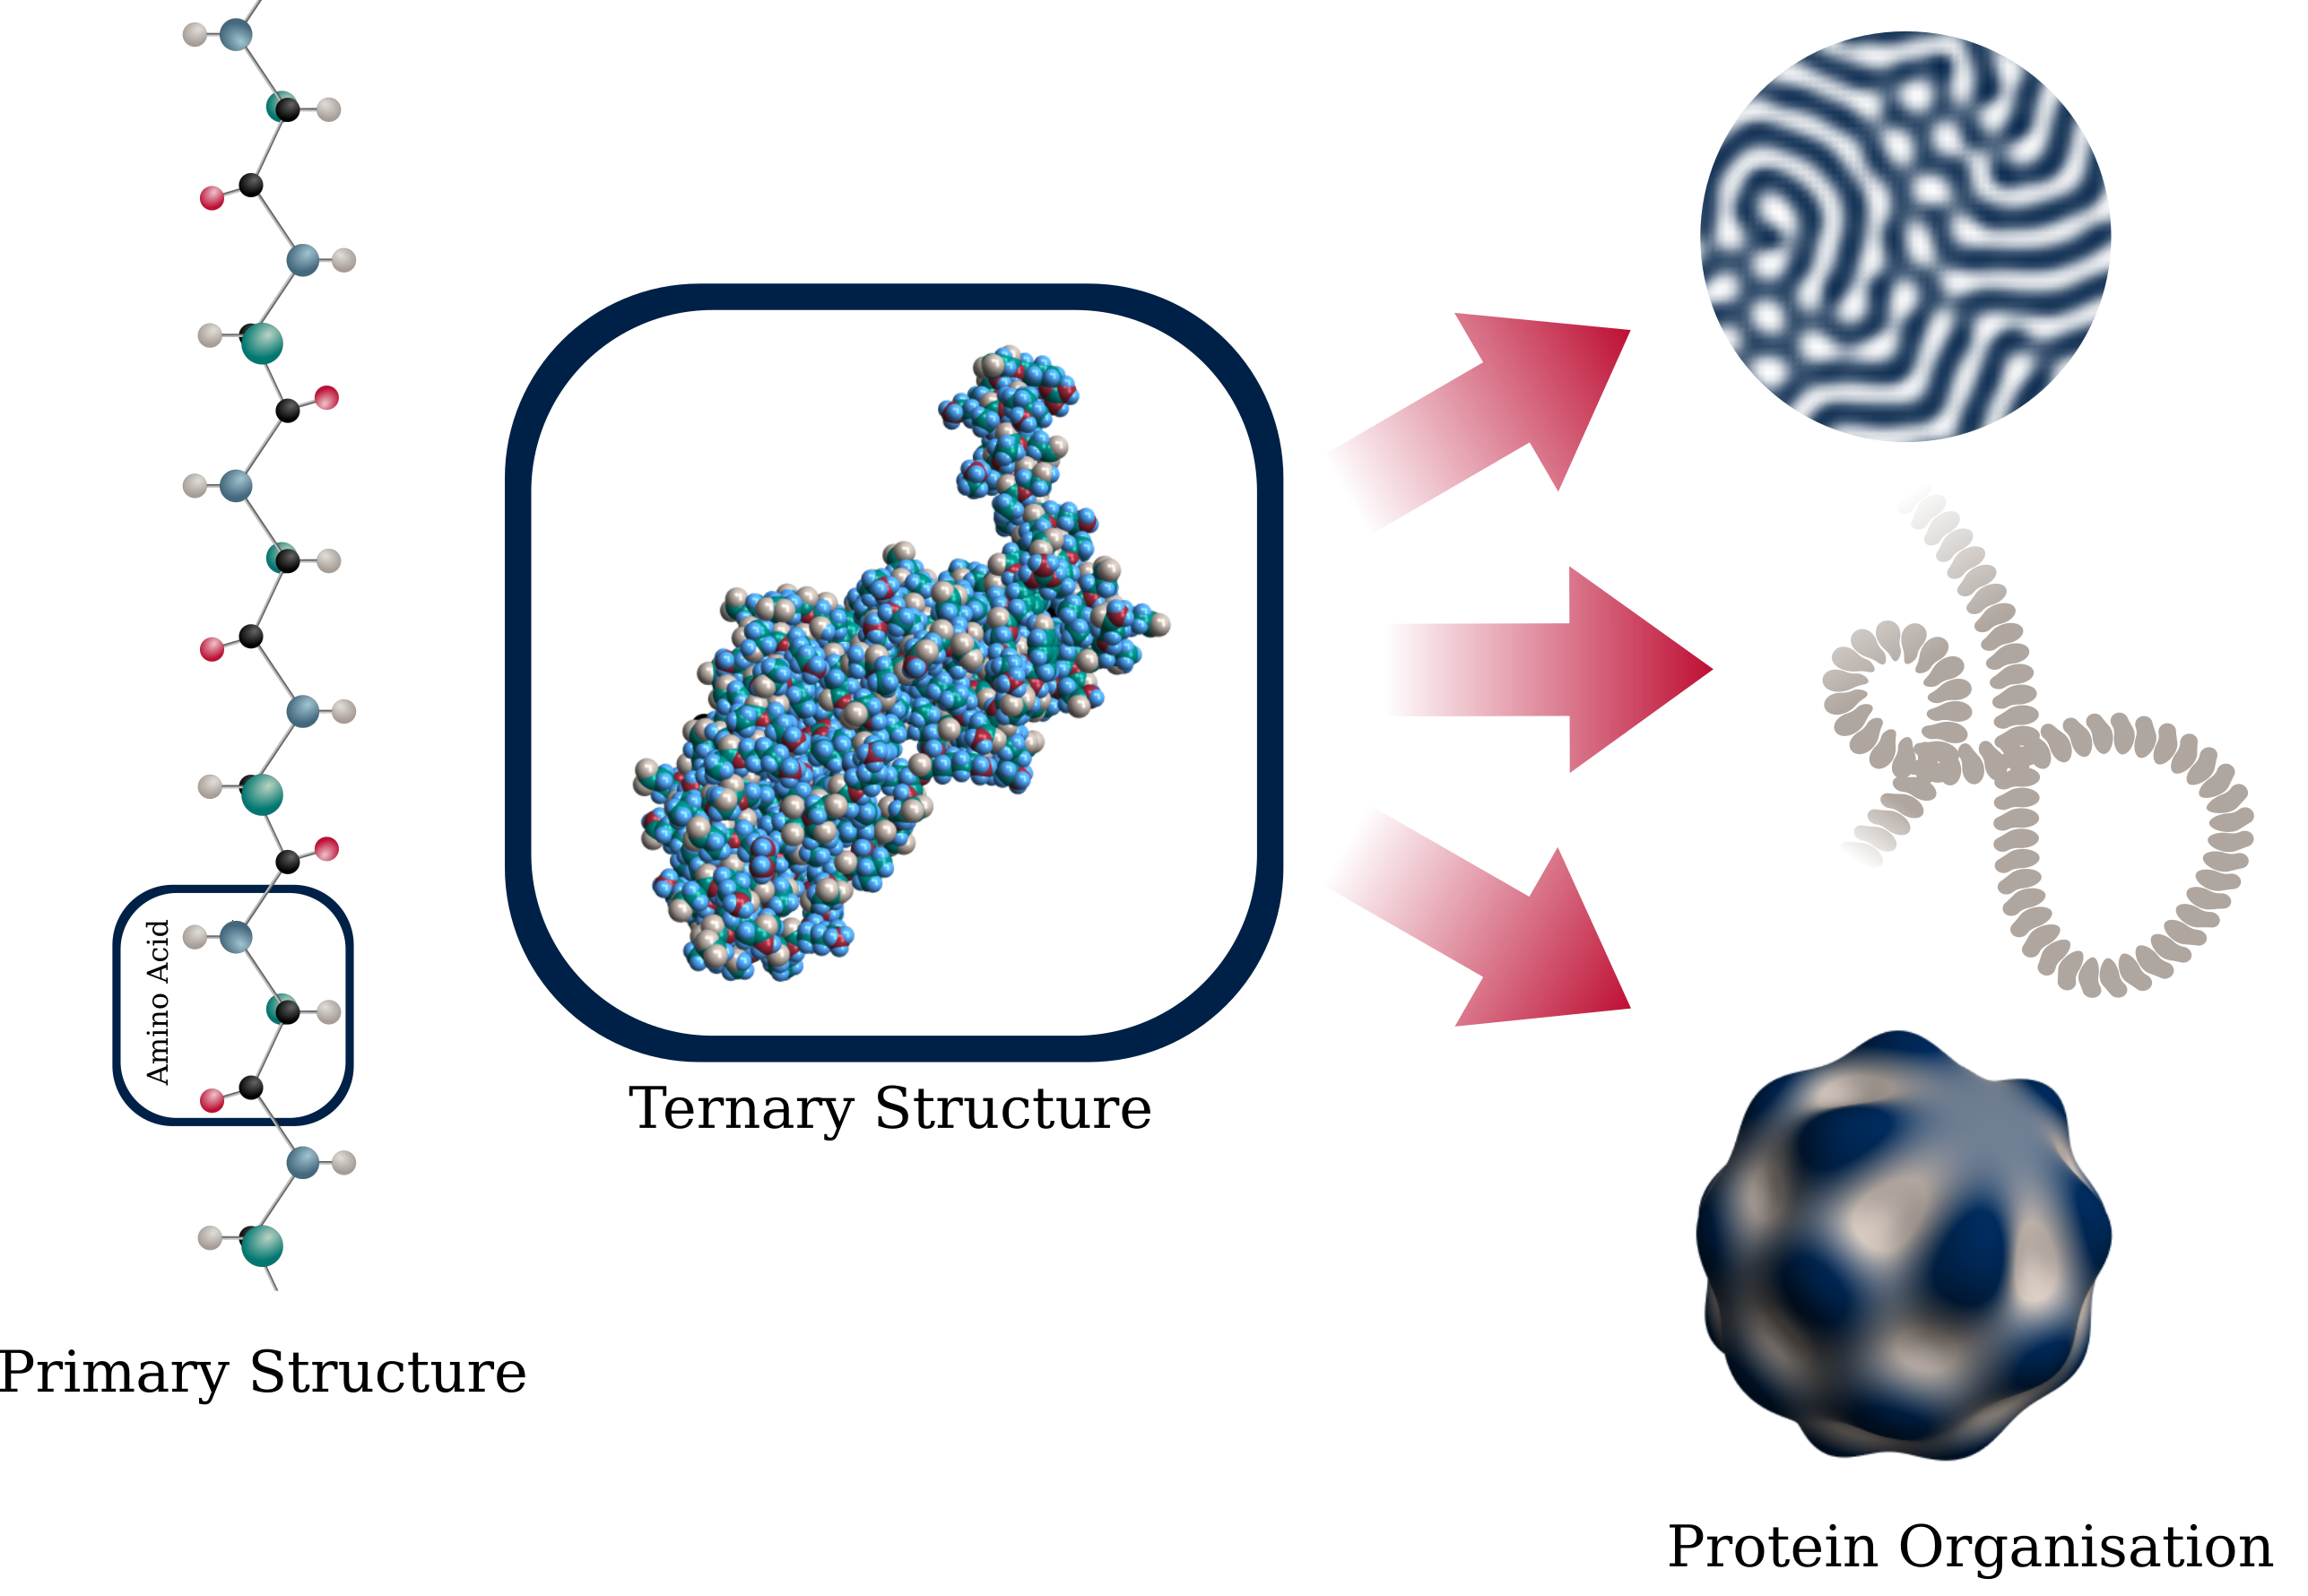
\includegraphics[width=1\textwidth]{figures/proteinLevels.png}
    \caption{The hierarchy of protein structure. Amino acids make proteins that then interact to form structures and patterns. The graphics show examples of protein organisation inspired by (top to bottom) reaction diffusion systems \cite{turing_chemical_1952}, fibrils \todo{ref} and curvature induced membrane patterning \cite{agudo-canalejo_pattern_2017}. The structure of the protein shown is generated from coordinates in the protein database, structure 1EZB, \cite{garrett_solution_1997}}
    \label{fig:1-proteinLevels}
\end{figure}


\section{Proteins in Health and Disease}

\section{Engineering Proteins}

synbio etc.

\section{Protein }
During my DPhil the development and release of AlphaFold changed the conversation around protein structure . AlphaFold is a neural network desigened to solve the problem of protein folding: learning the map from amino acid sequence (primary structure) to an atomistic description of the 3D shape (ternary structure). In 2021, AlphaFold became the first computational method to achieve accuracy on par with experimental structure determination. Since then, it has become an invaluable tool in arsenal of scientists trying to understand a variety of biological processes. Structure prediction can help to understand why a CRISP knockout might stop a molecule binding to a protein, elucidating unknown binding mechanisms, and engineering mutations to enhance binding affinity and catalytic rates. This model also represented a paradigm shift from mechanistic physics informed modelling to solve the folding problem to a deep learning approach. This was possible due to the extensive database of experimentally determined structures in the Protein Data Bank and the abundance of sequencing data from advanced sequencing technologies.

In this thesis, I have explored an alternative approach to protein engineering. Rather than considering changing the individual protein structure, I have explored mechanisms by which proteins can conspire to form structures that affect function. This collective organization often relates to protein structure; for instance, intrinsically disordered domains can drive equilibrium phase separation [and alphafold has helpd i think...]. However, my research demonstrates that the protein environment also plays a crucial role in tuning emergent phenomena. Varying monomer concentration in systems of aggregating proteins, adding solvent to a dense active mixture, or increasing the tension in a membrane filled with proteins are all examples of the rich parameter space that can be engineered when we begin to understand larger scale protein dynamics. 

The physics of these systems and mechanistic modelling remain central to research in this area. Recent studies have used AI etc. to determine the dynamics, but doesnt really give advice about coupleing them, or general downstream effects etc. Also need to determine whats important in each system (tbf AI could probable help with this). However more crucailly, in these cases the question is quite spceific. Here we cant quite do this, the question is less obvious...

What we can do is solve more sepcific question... reaction networks - Vincent + Antonis. But coupling everything together will give the best results...



The current suit of experimental data do not provide sufficient 

The question is less well posed. 

for example disordered regions of protein structure are hard to predict with alphaFold, but are more likely tro 
Intrinsically disordered proteins (pappu reference).
\cite{jumper_highly_2021}
Although not 

Used AI rather than physics based models

an  accuracy that the assessors considered competitive with that of experimental methods

The protein folding problem is now often refereed to as \textit{solved} and the application of \todo{AI} has shifted the focus from physically informed mechanistic models, into

\section{Abstracting and Modelling Proteins}

The space of amino acid chains and therefore of potential proteins is vast. There are \todo{potentially a calculation here?} The massive design space has been exploited by evolution to give a variety of 

Proteins are a fantastic model system for mathematicians and physicists to study. They are small enough to abstract as simple particles, but have sufficient complexity that they can maintain a plethora of reactions as described above. But more recently they can be engineered…

\section{How do proteins interact}

Protein organisation in health and disease

\section{Dump}

Refrerence Jaime’s dimer stuff, I like that PNAS paper

\section{Thesis Scope and Structure}

Each chapter in this thesis explores a different physical mechanism to drive protein organisation. I will introduce the background necessary to understand each mechanism and highlight specific aspects of these protein-protein interactions that have been previously understudied. Using a range of techniques, I will build mathematical models that incorporate this understudied features and study their effects on the resulting protein organisation, and ultimately how this can affect function or pathology. Below I provide a very brief summary of each system studied:
\begin{enumerate}
    \item \textbf{Catalysis Induced Phase Separation} Liquid-liquid phase separation can form droplets in mixtures of proteins and other components. The formation of these regions can be driven by equilibrium interactions between the components, but in this chapter I demonstrate that modelling chemically active components can give rise to fundamentally new phenomena. An enzymatic component can drive liquid-liquid phase separation without the interactions and this can subsequently affect overall reaction rates in the system.
    \item \textbf{Anisotropic Membrane Mediated Interactions} Proteins that bind to and bend biological membranes can generate elastic forces that act on other proteins in the membrane. These forces can generate structures and remodel the membrane. However, many of the proteins that bind in this way break radial symmetry and this changes their interactions, introducing an equilibrium separation and forming lattices of inclusions that can be controlled via the protein curvature or membrane tension.
    \item \textbf{Bounded clearance in Neurodegenerative Disease}\todo{could use actual chapter titles and enumerate with chapter numbers perhaps?} A plethora of neurodegenrative diseases are associated with aggregated proteins that are produced and removed in the brain. However, existing models ignore physical constraints that limits and bounds the rates at which these aggregated proteins can be removed. Including this key limit when modelling the aggregation kinetics can present a fundamentally new mechanism for the onset of disease which is consistent with recent experiments and can help design rational therapeutics.
\end{enumerate}